%!TEX program = xelatex
% 完整编译: xelatex -> biber/bibtex -> xelatex -> xelatex
\documentclass[lang=cn,a4paper,newtx,bibend=bibtex]{elegantpaper}
\usepackage{tikz}
\usepackage{pgfplots}

\title{Programming Report of Chapter 1}
\author{张志心 \ 混合2106}

\date{\zhdate{2023/09/30}}

% \qedhere to make the square straight after

\usepackage{array}
\usepackage{tcolorbox}

\newtcolorbox{prob}[1][]{
  colframe=gray,
  colback=white,
  boxrule=1.5pt, % 控制外边框线的宽度
  sharp corners, % 使用直角边框
  fonttitle=\bfseries,
  title=#1
}

\newcommand{\ccr}[1]{\makecell{{\color{#1}\rule{1cm}{1cm}}}}

\addbibresource[location=local]{reference.bib}

\begin{document}

\maketitle

\section{设计思路}

\subsection{函数类}

函数类作为一个抽象的模板类,其中 \lstinline[language=C++]{operator()} 函数为纯虚函数,
用于函数的求值运算,\lstinline[language=C++]{Diff()} 函数为求导运算,
(对于向量函数而言,即为求梯度运算)。

\begin{lstlisting}[language=C++]
  template <class Xtype, class Ytype = Xtype> 
  class Function{
  public:
      virtual Ytype operator() (const Xtype& x) const = 0;
      virtual Ytype Diff (const Xtype& x) const {custom_assert(0, "Diff() has not be designed\n");}
  };
\end{lstlisting}

为了简化求导的运算,
还对本次实验中使用的常见的 \texttt{F: double} $\to$ \texttt{double}
类型的函数的求导运算进行了特化,使用

\[
  f'(x) \simeq \dfrac{f(x+\epsilon)-f(x-\epsilon)}{2\epsilon}.
\]

作为导数的近似,取 \lstinline[language=C++]{10*std::numeric_limits<NUM>::epsilon()} 
作为 $\epsilon$ 的值。当继承类并未定义 \lstinline[language=C++]{Diff()} 函数时,
默认采用如下函数作为求导函数:

\begin{lstlisting}[language=C++]
  template<>
  NUM Function<NUM, NUM>::Diff (const NUM& x) const {
      // the default difference calculator
      return ((*this)(x+EPS_MIN)-(*this)(x-EPS_MIN))/(2*EPS_MIN);
  }
\end{lstlisting}

在使用时,需要定义一个具体的函数作为 \lstinline[language=C++]{class function} 的
继承,并定义其求值运算(必要的)和求导运算(可选择的)。
比如函数类 $f(x) = x - tan(x)$ 的定义如下:

\begin{lstlisting}[language=C++]
  class func : public Function<double, double>{
    public:
      double operator() (const double& x) const {
          return x-tan(x);
      }
      double Diff(const double& x) const {
          return 1-1/(sq(cos(x)));
      }
  };
\end{lstlisting}

\subsection{方程求解类}

\lstinline[language=C++]{class EquationSolver} 为方程求解基类,
其中只含有一个 \lstinline[language=C++]{solve()} 的纯虚函数。

代码实现见 \lstinline{EquationSolver.hpp},在使用时,请先引用该文件(\lstinline[language=C++]{#include "EquationSolver.hpp"})。

\subsubsection{Bisection Method}

\lstinline[language=C++]{class Bisection_Method: public EquationSolver}
为二分法的求解类,用于求解方程 $f(x) = 0$ 在初始区间上的解。其成员变量包括:求解函数 $f(x)$ 、
迭代初始区间 $[a,b]$ 、迭代终止条件 $\epsilon$ 和 $\delta$ 、以及最大的迭代次数
$Maxiter$。当以下任何一个条件不满足时,结束迭代:

\begin{equation*}
  \begin{cases}
    \vert f(\dfrac{a+b}{2})\vert \le \epsilon \\
    \vert a - b\vert \le \delta \\
    iter \le Maxiter.
  \end{cases}
\end{equation*}

二分法求解类的构造函数定义如下:

\begin{lstlisting}[language=C++]
  Bisection_Method(const Function<Type> &F, const Type &a, const Type &b, 
                    const NUM& eps = 1e-7, const NUM& delta = 1e-8, const int& Maxiter = 50) :
        F(F), a(a), b(b), Maxiter(Maxiter), eps(eps), delta(delta) {}
\end{lstlisting}

可以使用 \lstinline[language=C++]{Bisection_Method solver(f, a, b);} 构造一个
二分法求解实例(其中参数采用默认值),然后调用 \lstinline[language=C++]{solver.solve()} 来进行求解运算。 

\subsubsection{Newton Method}

\lstinline[language=C++]{class Newton_Method: public EquationSolver}
为牛顿法的求解类,用于求解方程 $f(x) = 0$ 在初始值附近的解。其成员变量包括:求解函数 $f(x)$ 、
初始值 $x_0$ 、迭代终止条件 $\epsilon$ 、以及最大的迭代次数
$Maxiter$。当以下任何一个条件不满足时,结束迭代:

\begin{equation*}
  \begin{cases}
    \vert f(x_n)\vert \le \epsilon \\
    iter \le Maxiter.
  \end{cases}
\end{equation*}

牛顿法求解类的构造函数定义如下:

\begin{lstlisting}[language=C++]
  Newton_Method(const Function<Type> &F, const Type &x0, 
                    const NUM& eps = 1e-7, const int& Maxiter = 50) :
        F(F), x0(x0), Maxiter(Maxiter), eps(eps){}
\end{lstlisting}

可以使用 \lstinline[language=C++]{Newton_Method solver(f, x0);} 构造一个
牛顿法求解实例(其中参数采用默认值),然后调用 \lstinline[language=C++]{solver.solve()} 来进行求解运算。 

\subsubsection{Secant Method}

\lstinline[language=C++]{class Secant_Method: public EquationSolver}
为割线法的求解类,用于求解方程 $f(x) = 0$ 在初始值附近的解。其成员变量包括:求解函数 $f(x)$ 、
初始值 $x_0,x_1$ 、迭代终止条件 $\epsilon$ 和 $\delta$ 、以及最大的迭代次数
$Maxiter$。当以下任何一个条件不满足时,结束迭代:

\begin{equation*}
  \begin{cases}
    \vert f(x_n)\vert \le \epsilon \\
    \vert x_n - x_{n-1} \vert \le \delta \\
    iter \le Maxiter.
  \end{cases}
\end{equation*}

割线法求解类的构造函数定义如下:

\begin{lstlisting}[language=C++]
  Secant_Method(const Function<Type> &F, const Type& x0, const Type& x1,
                const NUM& eps = 1e-7, const NUM& delta = 1e-8, const int& Maxiter = 50) :
          F(F), x0(x0), x1(x1), Maxiter(Maxiter), eps(eps), delta(delta){}
\end{lstlisting}

可以使用 \lstinline[language=C++]{Secant_Method solver(f, x0, x1);} 构造一个
割线法求解实例(其中参数采用默认值),然后调用 \lstinline[language=C++]{solver.solve()} 来进行求解运算。 


\section{求解结果}

\subsection{问题B}

设置 $\epsilon = 10^{-7}, \delta = 10^{-8}$ 二分法求解结果如下:

\begin{table}[htbp]
\begin{center}
\begin{tabular}{|c|c|c|c|c|c|}
  \hline
  $f(x)$ & $[a, b]$ & 近似解$x^*$ & $\vert f(x^*) \vert$ & 迭代次数 $iter$ & 终止区间长度 $b^*-a^*$ \\
  \hline
  $x^{-1} - \tan x$ & $[0, \pi/2]$ & 0.8603336024 & 0.0000000495 & 24 & 0.0000000936 \\
  \hline
  $x^{-1} - 2^x$ & $[0, 1]$ & 0.6411857605 & 0.0000000562 & 17 & 0.0000076294 \\
  \hline
  $2^{-x} + e^x + 2\cos x - 6$ & $[1, 3]$ & 1.8293836117 & 0.0000000400 & 22 & 0.0000004768 \\
  \hline
  $\frac{x^3+4x^2+3x+5}{2x^3-9x^2+18x-2}$ & $[0, 4]$ & 0.1178765632 & -94846963.165 & 29 & 0.0000000075 \\
  \hline
\end{tabular}
\end{center}
\end{table}

二分法没有办法正确求解第四个函数 $f(x) = \dfrac{x^3+4x^2+3x+5}{2x^3-9x^2+18x-2}$ 的根。
这是由于该函数的分子在 $[0,4]$ 上恒大于 $0$,而分母在 $[0,4]$ 上有一个零点,
导致二分法实际在求解的是分母的零点,而原函数该区间上没有零点,其在 $x\simeq 0.11788$ 处发散。

\begin{center}
\begin{figure}[htbp]
  \centering
  \begin{minipage}[b]{0.5\textwidth}
    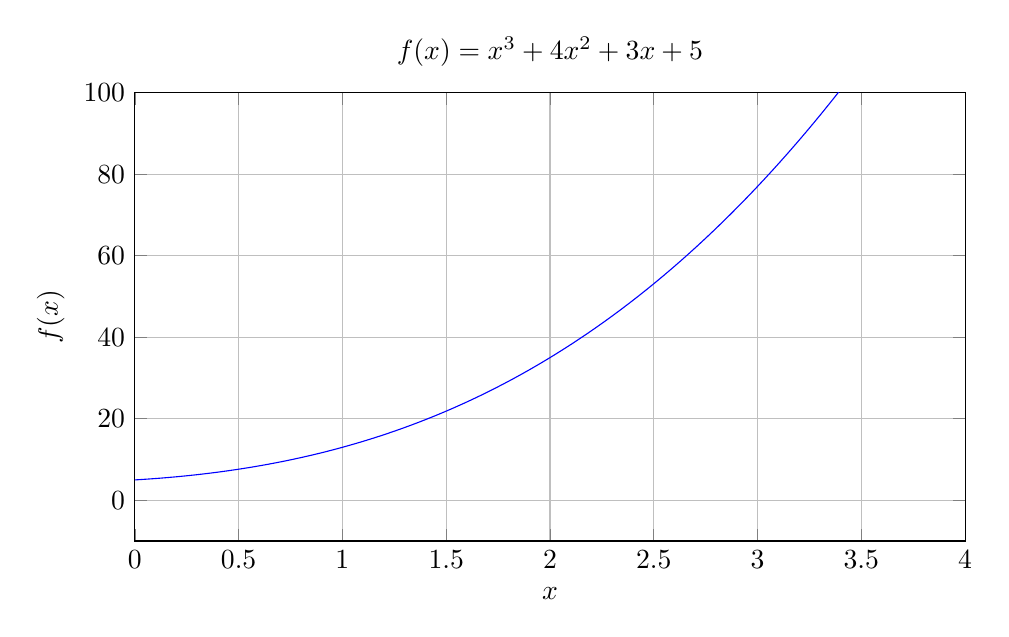
\begin{tikzpicture}
      \begin{axis}[
        xlabel={$x$},
        ylabel={$f(x)$},
        domain=0:4,
        samples=100,
        grid=major,
        width=1.0\textwidth,
        height=0.6\textwidth,
        xmin=0, xmax=4,
        ymin=-10, ymax=100,
        legend pos=north west,
        legend style={draw=none},
        title={$f(x) = x^3 + 4x^2 + 3x + 5$}
        ]
        \addplot[blue] {(x^3 + 4*x^2 + 3*x + 5)};
      \end{axis}
    \end{tikzpicture}
  \end{minipage}%
  \begin{minipage}[b]{0.5\textwidth}
    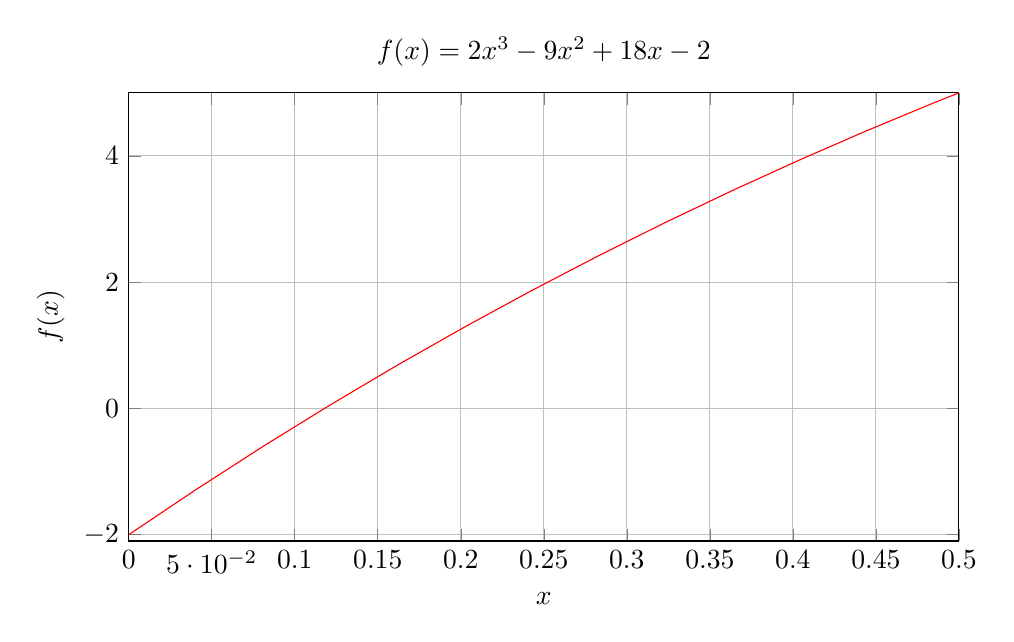
\begin{tikzpicture}
      \begin{axis}[
        xlabel={$x$},
        ylabel={$f(x)$},
        domain=0:4,
        samples=100,
        grid=major,
        width=1.0\textwidth,
        height=0.6\textwidth,
        xmin=0, xmax=0.5,
        ymin=-2.1, ymax=5,
        legend pos=north west,
        legend style={draw=none},
        title={$f(x) = 2x^3 - 9x^2 + 18x - 2$}
        ]
        \addplot[red] {2*x^3 - 9*x^2 + 18*x - 2};
        \draw [fill=red] (0.11787/0.5*50, 2.1/7.1*71) circle [radius=2pt];
        \node [anchor=west] at (0.11787/0.5*50, 2.1/7.1*71) {$x = 0.11788$};
      \end{axis}
    \end{tikzpicture}
  \end{minipage}
\end{figure}
\end{center}

\subsection{问题C}

即为求解 $f(x)=x-\tan x$ 的零点,$f'(x) = 1-\dfrac{1}{{\cos x}^2}$。

设置 $\epsilon = 10^{-7}$,牛顿法求解结果如下:

\begin{table}[htbp]
	\centering
	\begin{tabular}{|c|c|c|c|c|}
		\hline
    $f(x)$ & $x_0$ & 近似解$x^*$ & $\vert f(x^*) \vert$ & 迭代次数 $iter$ \\
    \hline
		\multirow{2}*{$f(x)=x-\tan x$} & 4.5 & 4.4934094579 & 0.0000000000 & 3 \\
		\cline{2-5}
		~ & 7.7 & 7.7252518369 & 0.0000000000 & 4 \\
		\hline
	\end{tabular}
\end{table}

\subsection{问题D}

使用割线法求解 $\sin(\frac{x}{2})-1$, $e^x-\tan x$, $x^3-12x^2+3x+1$,
设置迭代终止条件 $\epsilon=10^{-7}, \delta=10^{-8}$。
为每一个函数都设置了不同的初始值 $x_0,x_1$,得到结果如下表所示。

\begin{table}[htbp]
	\centering
	\begin{tabular}{|c|c|c|c|c|c|c|}
		\hline
    $f(x)$ & $x_0$ & $x_1$ & 近似解$x^*$ & $\vert f(x^*) \vert$ & 迭代次数 $iter$ & $\vert x_n-x_{n-1}\vert$ \\
    \hline
		\multirow{2}*{$f(x)=\sin(\frac{x}{2})-1$} & 0 & $\frac{\pi}2$ & 3.1409322315 & .0000000545 & 16& 0.0004081633\\
		\cline{2-7}
		~ & 14 & 15 & 15.7074076584 & 0.0000000386 & 15& 0.0003433855\\
		\hline
    \multirow{2}*{$f(x)=e^x-\tan x$} & 1 & 1.4 & 1.3063269404 & 0.0000000000 & 9& 0.0000000151\\
		\cline{2-7}
		~ & -2.8 & -3.1 & -3.0964122941 & 0.0000000103 &2 & 0.0001338862 \\
		\hline
    \multirow{2}*{$f(x)=x^3-12x^2+3x+1$} & 0 & -0.5 & -0.1886854043 & 0.0000000063 & 6 & 0.0000019974 \\
		\cline{2-7}
		~ & 8 & 9 & 11.7371421792 & 0.0000000004 & 10 & 0.0000001458 \\
		\hline
	\end{tabular}
\end{table}

可以发现,不同的初始值会导致不同的求解结果。
这是因为函数有不止一个零点,而割线法更倾向于找到离初始点近的零点。
下为三个函数的函数图像:

\begin{figure}[htbp]
\centering
\begin{minipage}{0.33\textwidth}
% Plot 1: sin(x/2) - 1
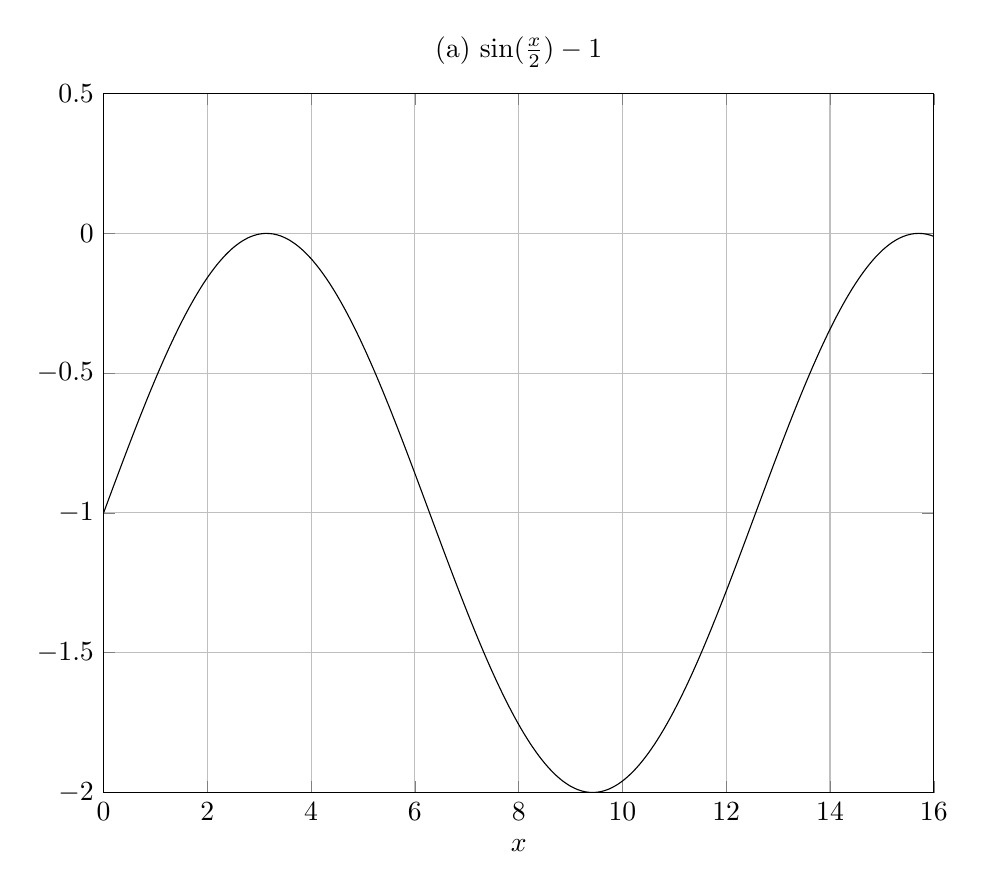
\begin{tikzpicture}
\begin{axis}[
    width=\textwidth,
    xmin=0, xmax=16,
    ymin=-2, ymax=0.5,
    domain=0:15,
    smooth,
    samples=200,
    xlabel={$x$},
    grid=major,
    title={(a) $\sin(\frac{x}{2}) - 1$}
]
\addplot[domain=-10:20, samples=200]{sin(deg(x/2))-1};
\end{axis}
\end{tikzpicture}
\end{minipage}
\begin{minipage}{0.33\textwidth}
% Plot 2: e^x - tan(x)
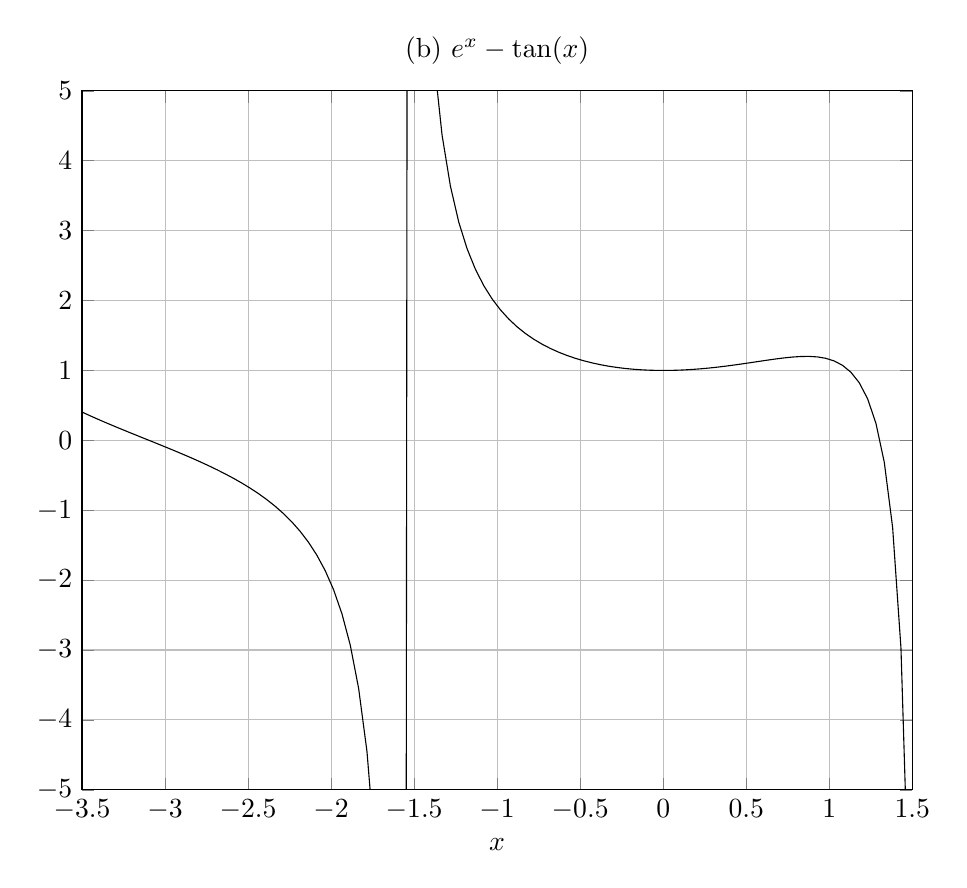
\begin{tikzpicture}
\begin{axis}[
    width=\textwidth,
    xmin=-3.5, xmax=1.5,
    ymin=-5, ymax=5,
    xlabel={$x$},
    grid=major,
    title={(b) $e^x - \tan(x)$}
]
\addplot[domain=-5:5, samples=200]{exp(x) - tan(deg(x))};
\end{axis}
\end{tikzpicture}
\end{minipage}
\begin{minipage}{0.33\textwidth}
% Plot 3: x^3 - 12x^2 + 3x + 1
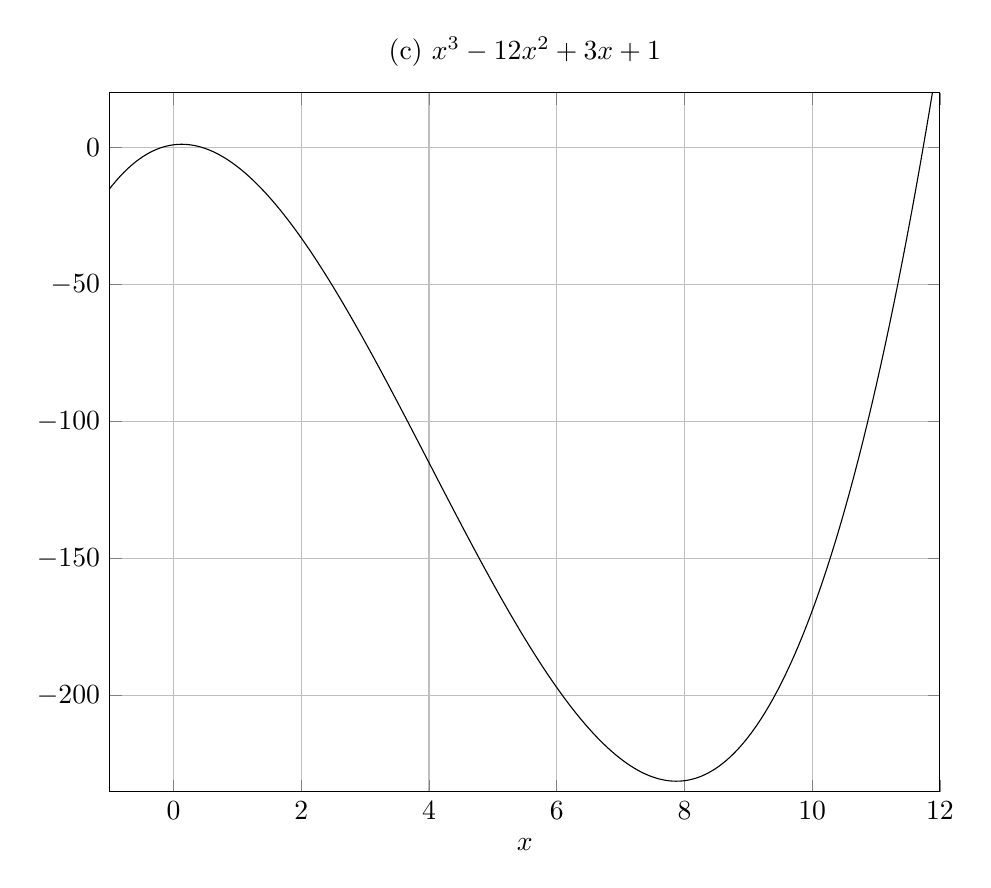
\begin{tikzpicture}
\begin{axis}[
    width=\textwidth,
    xmin=-1, xmax=12,
    ymin=-235, ymax=20,
    domain=-1:12,
    smooth,
    samples=200,
    xlabel={$x$},
    grid=major,
    title={(c) $x^3 - 12x^2 + 3x + 1$}
]
\addplot[domain=-5:15, samples=200]{x^3 - 12*x^2 + 3*x + 1};
\end{axis}
\end{tikzpicture}
\end{minipage}
\end{figure}


\subsection{问题E}

求解方程:

\[
  f(h)=V-L\bigg[\dfrac{1}{2}\pi r^2-r^2\arctan\dfrac{h}r-h\sqrt{r^2-h^2}\bigg] = 0.
\]

对函数 $f(h)$ 进行求导得到:

\[
  f'(h) = L\bigg[\dfrac{r}{\sqrt{1-(h/r)^2}}+\dfrac{x^2}{\sqrt{r^2-h^2}}+\sqrt{r^2-h^2}\bigg].
\]

问题所求水深即为 $r-h$。

代入 $V=12.4, L = 10, r = 1$,使用二分法、牛顿法、割线法求解结果如下:

\begin{table}[htbp]
	\centering
	\begin{tabular}{|c|c|c|c|c|c|c|c|}
		\hline
    Method & 初始条件 & 近似解$x^*$ & $\vert f(x^*) \vert$ & 迭代次数 $iter$ & $\epsilon$ & $\delta$ \\
    \hline
		Bisection & $[a,b]=[0,r]$ & 0.1640625000 & 0.0414932414 & 6 & $10^{-7}$ & 0.02\\
		\hline
    Newton& $x_0 = 0$ & 0.1653981634 & 0.0151449150 & 1  & $0.01\times 20$ & ~ \\
		\hline
    Secant & $x_0 = 0, x_1 = r$ & 0.1662278952 &  0.0012200043 & 3 &  $10^{-7}$ & $\frac12[(\frac{0.01}{0.547})^{0.618}-0.01]$ \\
		\hline
	\end{tabular}
\end{table}

最后,使用 Bisection 法,Newton 法,Secant 法得到的问题的答案分别为 0.8359375、0.8346018366、0.8337721048。
\newpage
备注:关于 $\delta$ 和 $\epsilon$ 的选取问题,

\begin{enumerate}
  \item 对于二分法,$\big\vert\dfrac{a_n+b_n}2-x^*\big\vert\le \dfrac12\big\vert a_n - b_n\big\vert$,所以将 $\delta$ 设置为$2\times 0.01$;
  \item 对于牛顿法,考虑在 $x^*$ 处 Taylor 展开:
        \[
          f(x_n)\simeq f(x^*)+(x_n-x^*)f'(x^*)
        \Rightarrow \bigg\vert x_n-x^*\bigg\vert \le \bigg \vert\dfrac{ f(x_n)}{f'(x^*)} \bigg\vert.
        \]
        根据估计,函数在零点处导数约为 20,因此取 $\epsilon = 20\times 0.01$,
        事实上,还可以为牛顿法增加一个 $\delta$ 项,然而这样会增加其计算负担,
        牛顿法的效率通常很高,精确性也很好,所以一般不需要增加迭代终止条件;
  \item 对于割线法的收敛性,有
        \begin{equation*}
          \begin{aligned}
          \vert x_n-x^* \vert &\le M{\vert x_{n-1} - x^{*}\vert}^{1.618} = M(-x_n + x_{n-1} + x_n - x^{*})^{1.618}. \\
          \delta &= M (\delta + 0.01)^{1.618} \Rightarrow \delta = (\frac{0.01}{M})^{0.618}-0.01.
        \end{aligned}
        \end{equation*}
        取 $M = \bigg\vert \frac{f''(x^*)}{f'(x^*)}\bigg\vert$ 作为其近似值,并且为整个式子
        增加一个 $\dfrac{1}{2}$ 的因子,得到 $\delta$ 如上表所示。
\end{enumerate}

% Solving Problem E with : V = 12.4, L = 10, r = 1
% --------------------Using Bisection Method------------------------
% Iteration times = 6
% Approximate root = 0.1640625000
% Function value = -0.0414932414
% Norm(b-a) = 0.0156250000
% ------------------------------------------------------------------
% --------------------Using Newton Method---------------------------
% Iteration times = 1
% Approximate root = 0.1653981634
% Function value = -0.0151449150
% Norm of Derivative = 20.0000000000
% ------------------------------------------------------------------
% --------------------Using Secant Method---------------------------
% Using Secant Method:
% Iteration times = 3
% Approximate root = 0.1662278952
% Function value = 0.0012200043
% Norm(x(k)-x(k-1)) = 0.0153874090
% ------------------------------------------------------------------

\subsection{问题F}

该问题需要把角度转化为弧度制,记 $k = \dfrac{\pi}{180}$。求解方程如下:

\[
  f(x)=A\sin{kx}\cos{kx}+B\sin^2{kx}-C\cos{kx}-E\sin{kx} = 0.
\]
\[
  f'(x)=k\bigg[A(\cos^2{kx}-\sin^2{kx})+2B\sin{kx}\cos{kx}+C\sin{kx}-E\cos{kx}\bigg].
  %Pi/180*(A*(sq(co)-sq(si))+B*(2*si*co)+C*si-E*co);
\]

(a) 和 (b) 使用牛顿法,采用了不同的参数值($D = 55, 30$),求解结果如下:

% Solving Problem F(a) : x0=33, l = 89, h = 49, D = 55, beta1 = 11.5
% --------------------Using Newton Method---------------------------
% Iteration times = 2
% Approximate root = 32.9721748224
% Function value = 0.0000000000
% Norm of Derivative = 0.9129412717
% ------------------------------------------------------------------
% Solving Problem F(b) : x0=33, l = 89, h = 49, D = 30, beta1 = 11.5
% --------------------Using Newton Method---------------------------
% Iteration times = 2
% Approximate root = 33.1689038218
% Function value = 0.0000000013
% Norm of Derivative = 0.9140901657


\begin{table}[htbp]
	\centering
	\begin{tabular}{|c|c|c|c|c|c|}
		\hline
    $x_0$ & 近似解$x^*$ & $\vert f(x^*) \vert$ & 迭代次数 $iter$ & $\epsilon$ \\
    \hline
		$33^\circ$ & $32.9721748224^\circ$ & 0.0000000000 & 2 & $10^{-7}$\\
		\hline
    $33^\circ$ & $33.1689038218^\circ$ & 0.0000000013 & 2 & $10^{-7}$\\
		\hline
	\end{tabular}
\end{table}

对于 (c) 题,在 $[0^\circ, 160^\circ]$ 中以 $10^\circ$ 为间距取了若干组 $x_0,x_1$ 作初始值,
可以发现不同的初始值将会收敛到不同的零点,具体结果如下:

\begin{center}
  \begin{tabular}{|c|c|c|c|c|}
  \hline
  \textbf{$x_0$} & \textbf{$x_1$} & 近似解$x^*$ & $\vert f(x^*) \vert$ & 迭代次数 $iter$  \\
  \hline
  $0^\circ$ & $10^\circ$ & $11.4999999493^\circ$ & 0.0000000586 & 8 \\
  $10^\circ$ & $20^\circ$ & $32.9721748162^\circ$ & 0.0000000057 & 6 \\
  $20^\circ$ & $30^\circ$ & $32.9721748224^\circ$ & 0.0000000000 & 5 \\
  $30^\circ$ & $40^\circ$ & $32.9721748157^\circ$ & 0.0000000061 & 4 \\
  $40^\circ$ & $50^\circ$ & $32.9721748224^\circ$ & 0.0000000000 & 5 \\
  $50^\circ$ & $60^\circ$ & $32.9721748224^\circ$ & 0.0000000000 & 5 \\
  $60^\circ$ & $70^\circ$ & $32.9721748225^\circ$ & 0.0000000001 & 6 \\
  $70^\circ$ & $80^\circ$ & $11.4999999999^\circ$ & 0.0000000001 & 7 \\
  $80^\circ$ & $90^\circ$ & $216867.0278251776^\circ$ & 0.0000000000 & 13 \\
  $90^\circ$ & $100^\circ$ & $1407.0278251776^\circ$ & 0.0000000001 & 8 \\
  $100^\circ$ & $110^\circ$ & $147.0278252723^\circ$ & 0.0000000452 & 8 \\
  $110^\circ$ & $120^\circ$ & $147.0278251774^\circ$ & 0.0000000001 & 6 \\
  $120^\circ$ & $130^\circ$ & $147.0278251735^\circ$ & 0.0000000019 & 6 \\
  $130^\circ$ & $140^\circ$ & $147.0278251776^\circ$ & 0.0000000000 & 6 \\
  $140^\circ$ & $150^\circ$ & $147.0278251767^\circ$ & 0.0000000004 & 5 \\
  $150^\circ$ & $160^\circ$ & $147.0278251356^\circ$ & 0.0000000200 & 7 \\
  \hline
  \end{tabular}
  \end{center}

可以发现,其中 $147^\circ$ 与 $33^\circ$ 两个恰好互补,前者恰好是车从左边上右边的坡的对称情景。

割线法的结果与初值点的选取有很大的关系,一般情况下,
割线法会容易偏向于找到初值点附近零点,这是基于每次求割线后与坐标轴的交点
一般不会离当前两个点太远,若在初值点附近存在零点,
则容易收敛到附近的零点上。

然而也会有特殊的情况,比如当割线斜率的绝对值太小时,割线与坐标轴的交点离当前的两个点就会很远。

进一步的,考虑割线法的收敛性质:

\[
  \vert x_n - x^* \vert \le M \vert x_{n-1}-x^* \vert \vert x_{n-2} - x^*\vert
\]

其中,$M = \dfrac{\max_{x\in \mathcal{B}}\vert f''(x)\vert}{2\min_{x\in \mathcal{B}} \vert f'(x) \vert}, 
\mathcal{B} = [x^*-\delta, x^*+\delta], \delta = \max(\vert x_1 - x^*\vert, \vert x_0 - x^*\vert)$,

当 $M$ 充分小的时候,一定会收敛到 $x^*$,否则 $\{x_n\}$ 就可能会收敛到其他零点,甚至不收敛。

  
  
\nocite{*}
\printbibliography[heading=bibintoc, title=\ebibname]

% \appendix
% % \appendixpage
% \addappheadtotoc

\end{document}
